%!TEX root = ../Thesis.tex
%% Basierend auf TeXnicCenter-Vorlage von Mark Müller
%%                      Willi Nüßer
%%                      Waldemar Penner     
%%                      Ulrich Reus
%%                      Frank Plass
%%                      Oliver Tribeß 
%%                      Daniel Hintze     
%%%%%%%%%%%%%%%%%%%%%%%%%%%%%%%%%%%%%%%%%%%%%%%%%%%%%%%%%%%%%%%%%%%%%%%

% Wählen Sie die Optionen aus, indem Sie % vor der Option entfernen  
% Dokumentation des KOMA-Script-Packets: scrguide

%%%%%%%%%%%%%%%%%%%%%%%%%%%%%%%%%%%%%%%%%%%%%%%%%%%%%%%%%%%%%%%%%%%%%%%
%% Optionen zum Layout des Artikels                                  %%
%%%%%%%%%%%%%%%%%%%%%%%%%%%%%%%%%%%%%%%%%%%%%%%%%%%%%%%%%%%%%%%%%%%%%%%
\documentclass[%
paper=A4,         % alle weiteren Papierformat einstellbar
fontsize=12pt,    % Schriftgröße (12pt, 11pt (Standard))
BCOR12mm,         % Bindekorrektur, bspw. 1 cm
DIV14,            % breiter Satzspiegel
parskip=half*,    % Absatzformatierung s. scrguide 3.1
headsepline,      % Trennline zum Seitenkopf  
%footsepline,     % Trennline zum Seitenfuß
%normalheadings,  % Überschriften etwas kleiner (smallheadings)
listof=totoc,     % Tabellen & Abbildungsverzeichnis ins Inhaltsverzeichnis      
%bibtotoc,        % Literaturverzeichnis im Inhalt 
%draft            % Überlangen Zeilen in Ausgabe gekennzeichnet
footinclude=false,% Fußzeile in die Satzspiegelberechnung einbeziehen 
headinclude=true, % Kopfzeile in die Satzspiegelberechnung einbeziehen 
final             % draft beschleunigt die Kompilierung
]
{scrartcl}

%\setuptoc{toc}{totoc} % Inhaltsverzeichnis ins Inhaltsverzeichnis

% Neue Deutsche Rechtschreibung und Deutsche Standardtexte
\usepackage[ngerman]{babel} 

% Umlaute können verwendet werden
\usepackage[utf8]{inputenc}   

% Echte Umlaute
\usepackage[T1]{fontenc} 

% Latin Modern Font, Type1-Schriftart für nicht-englische Texte
\usepackage{lmodern} 

% 1/2-zeiliger Zeilenabstand
\usepackage[onehalfspacing]{setspace}

% Für die Defenition eigener Kopf- und Fußzeilen
\usepackage{fancyhdr} 

% Für die Verwendung von Grafiken
\usepackage[pdftex]{graphicx}

% Bessere Tabellen
\usepackage{tabularx}

% Für die Befehle \toprule, \midrule und \bottomrule, z.B. in Tabellen 
\usepackage{booktabs}

% Erlaubt die Benutzung von Farben
\usepackage{color}

% Links im PDF
\usepackage{hyperref}

% Verbessertes URL-Handling mit \url{http://...}
\usepackage{url}

% Listen ohne Abstände \begin{compactlist}...\end{compactlist}
\usepackage{paralist} 

% Ausgabe der aktuellen Uhrzeit für die Draft-Versionen
\usepackage{datetime}

% Deutsche Anführungszeichen
\usepackage[babel,german=quotes]{csquotes}

% Verbessert das Referenzieren von Kapiteln, Abbildungen etc.
\usepackage[german,capitalise]{cleveref}

% Konfiguration der Abbildungs- und Tabellenbezeichnungen
\usepackage[format=hang, font={footnotesize, sf}, labelfont=bf, justification=raggedright,singlelinecheck=false]{caption}

% Verbessert die Lesbarkeit durch Mikrotypografie
\usepackage[activate={true,nocompatibility},final,tracking=true,kerning=true,spacing=true,factor=1100,stretch=10,shrink=10]{microtype}  

% Zitate und Quellenverzeichnis
\usepackage[
    style=authoryear,         % Zitierstil
    firstinits=false,         % false = Vornamen werden ausgeschrieben
    natbib=true,
    urldate=long,             % "besucht am" - Datum
    %url=false,
    date=long,                
    dashed=false, 
    maxcitenames=3,           % max. Anzahl Autorennamen in Zitaten
    maxbibnames=99,           % max. Anzahl Autorennamen im Quellenverzeichnis
    %backend=bibtex           % Ggf. für ältere Distributionen bibtex verwenden
]{biblatex}

% Bibliograpthy
\bibliography{library/library}

% Keine Einrückung bei einem neuen Absatz
\parindent 0pt 

% Ebenentiefe der Nummerierung
\setcounter{secnumdepth}{3}

% Gliederungstiefe im Inhaltsverzeichnis 
\setcounter{tocdepth}{3} 

% Tabellen- und Abbildungsverzeichnis mit Bezeichnung:
\usepackage[titles]{tocloft}
\renewcommand*\cftfigpresnum{Abbildung~}
\renewcommand*\cfttabpresnum{Tabelle~}
\renewcommand{\cftfigaftersnum}{:}
\renewcommand{\cfttabaftersnum}{:}
\settowidth{\cftfignumwidth}{\cftfigpresnum 99~\cftfigaftersnum}
\settowidth{\cfttabnumwidth}{\cfttabpresnum 99~\cftfigaftersnum}

% Style für Kopf- und Fußzeilenfelder
\pagestyle{fancy}
\fancyhf{}
\fancyhead[R]{\leftmark}
\fancyfoot[R]{\thepage} 
\renewcommand{\sectionmark}[1]{\markboth{#1}{#1}} 
\fancypagestyle{plain}{}

% Macro für Quellenangaben unter Abbildungen und Tabellen
\newcommand{\source}[1]{{\vspace{-1mm}\\\footnotesize\textsf{\textbf{Quelle:}} \textsf{#1}\par}}

% Sourcecode-Listings
\usepackage{listings}

% Bestimmte Warnungen unterdrücken
% siehe http://tex.stackexchange.com/questions/51867/koma-warning-about-toc
\usepackage{scrhack} 

% Anpassungen der Formatierung an Eclipse-Aussehen 
% http://jevopi.blogspot.de/2010/03/nicely-formatted-listings-in-latex-with.html
%\definecolor{sh_comment}{rgb}{0.12, 0.38, 0.18 } %adjusted, in Eclipse: {0.25, 0.42, 0.30 } = #3F6A4D
%\definecolor{sh_keyword}{rgb}{0.37, 0.08, 0.25}  % #5F1441
%\definecolor{sh_string}{rgb}{0.06, 0.10, 0.98} % #101AF9
% Für Druckausgabe sollte alles schwarz sein
\definecolor{sh_comment}{rgb}{0.0, 0.0, 0.0 }
\definecolor{sh_keyword}{rgb}{0.0, 0.0, 0.0 }
\definecolor{sh_string}{rgb}{0.0, 0.0, 0.0 }

\lstset{ %
  language=Java,
  basicstyle=\small\ttfamily,
  fontadjust, 
  xrightmargin=1mm,
  xleftmargin=5mm,
  tabsize=2,
  columns=flexible,
  showstringspaces=false,
  rulesepcolor=\color{black},
  showspaces=false,showtabs=false,tabsize=2,
  stringstyle=\color{sh_string},
  keywordstyle=\color{sh_keyword}\bfseries,
  commentstyle=\color{sh_comment}\itshape,
  captionpos=t,
  lineskip=-0.3em
}

\renewcommand{\lstlistingname}{Listing}
\renewcommand\lstlistlistingname{Listingverzeichnis}

\makeatletter
\def\l@lstlisting#1#2{\@dottedtocline{1}{0em}{1em}{\lstlistingname\space{#1}}{#2}}
\makeatother

% Anhangsverzeichnis
\usepackage[nohints]{minitoc} %Anhangsverzeichnis

\makeatletter
\newcounter{fktnr}\setcounter{fktnr}{0}
\newcounter{subfktnr}[fktnr]\setcounter{subfktnr}{0}

\renewcommand\thesubfktnr{\arabic{fktnr}.\thefktnr}
\newcounter{anhangcounter}
\newcommand{\blatt}{\stepcounter{anhangcounter}}

\newcommand{\anhang}[1]{\setcounter{anhangcounter}{0}\refstepcounter{fktnr}
\addcontentsline{fk}{subsection}{Anhang~\thefktnr: \hspace*{1em}#1}
\subsection*{{Anhang~\thefktnr \hspace*{1em} #1 \hspace*{-1em}}}
}

\newcommand{\subanhang}[1]{\setcounter{anhangcounter}{0}\refstepcounter{subfktnr}
\addcontentsline{fk}{subsubsection}{Anhang~\thesubfktnr: \hspace*{1em}#1}
\subsubsection*{{Anhang~\thesubfktnr \hspace*{1em} #1 \hspace*{-1em}}}
}

\newcommand{\anhangsverzeichnis}{\mtcaddsection{\subsection*{Anhangsverzeichnis \@mkboth{FKT}{FKT}}}\@starttoc{fk}\newpage}

% Abkürzungsverzeichnis
\usepackage[acronym,         % create list of acronyms
            nonumberlist,
            toc, 
            section,
            nomain,          % don't need main glossary for this example
            hyperfirst=false,% don't hyperlink first use
            sanitize=none    % switch off sanitization as description
            ]{glossaries}
            \newglossarystyle{mylist}{%
\glossarystyle{long}% base this style on the list style
\renewcommand*{\glossaryentryfield}[5]{%
    \glsentryitem{##1}\textbf{##2} & ##3 \\}%
}

\newacronym{AES}{AES}{Advanced Encryption Standard}
\newacronym{AI}{AI}{Artificial Intelligence}
\newacronym{AOA}{AOA}{Angle of Arrival}
\newacronym{API}{API}{Application Programming Interface}
\newacronym{ATM}{ATM}{Automated Teller Machine}
\makeglossaries\makeglossaries

%%%%%%%%%%%%%%%%%%%%%%%%%%%%%%%%%%%%%%%%%%%%%%%%%%%%%%%%%%%%%%%%%%%%%%%
%% Parameter - Hier auf die eigene Arbeit anpassen
%%%%%%%%%%%%%%%%%%%%%%%%%%%%%%%%%%%%%%%%%%%%%%%%%%%%%%%%%%%%%%%%%%%%%%%

\newcommand{\dokumententyp}{Bachelorthesis}
\newcommand{\abgabedatum}{\today} 
\newcommand{\ort}{Paderborn} 
\newcommand{\koorperationsunternehmen}{Unternehmen GmbH}
\newcommand{\dokumententitel}{Konzeption und prototypische Realisierung einer \dokumententyp{} mit {\LaTeX}}
\newcommand{\dokumentenautor}{Max Mustermann}
\newcommand{\dokumentenautoradress}{Musterweg 123\\33102 Paderborn}
\newcommand{\dokumentenpruefer}{Prof. Dr. Weis-Alles\\Prof. Dr. Besser}

%%%%%%%%%%%%%%%%%%%%%%%%%%%%%%%%%%%%%%%%%%%%%%%%%%%%%%%%%%%%%%%%%%%%%%%

\hypersetup{
  colorlinks=false,
  pdfborder={0 0 0},
  pdftitle=\dokumententitel,
  pdfauthor=\dokumentenautor
} 

\begin{document}

% Römische Seitennummerierung
\pagenumbering{Roman}
 
%%%%%%%%%%%%%%%%%%%%%%%%%%%%%%%%%%%%%%%%%%%%%%%%%%%%%%%%%%%%%%%%%%%%%%%
%% Titelseite
%%%%%%%%%%%%%%%%%%%%%%%%%%%%%%%%%%%%%%%%%%%%%%%%%%%%%%%%%%%%%%%%%%%%%%%

%!TEX root = ../Thesis.tex

\begin{titlepage}

\begin{center}


\includegraphics[scale=1.20]{img/fhdw}\\

\ort\\

\vspace{.7cm}

\large{\bfseries\dokumententyp}

~\vspace{.1cm}\\

\LARGE{\dokumententitel}

~\vspace{.1cm}\\

\large{

Prüfer:\vspace{1mm}\\

\dokumentenpruefer

\vspace{1cm}

Verfasser:\\\vspace{1mm}

\dokumentenautor\\
\dokumentenautoradress


\begin{center}
    \begin{tabular}{rcl} 
       Matrikelnummer &:& \matnummer\\
       \vspace{1cm}\\
       Studiengang &:& \studiengang \\ 
       Spezialisierungsbereich &:& \spezialisierungsbereich \\ 
    \end{tabular}
\end{center} 


\vspace{1.5cm}

Abgabetermin:\\

\abgabedatum

}

\end{center}


\end{titlepage}



%%%%%%%%%%%%%%%%%%%%%%%%%%%%%%%%%%%%%%%%%%%%%%%%%%%%%%%%%%%%%%%%%%%%%%%
%% Draft-Einstellungen
%%
%% Für die finale Version auskommentieren!
%%%%%%%%%%%%%%%%%%%%%%%%%%%%%%%%%%%%%%%%%%%%%%%%%%%%%%%%%%%%%%%%%%%%%%%
\fancyhead[L]{\color{red} Stand: \today~-~\currenttime}

%%%%%%%%%%%%%%%%%%%%%%%%%%%%%%%%%%%%%%%%%%%%%%%%%%%%%%%%%%%%%%%%%%%%%%%
%% Verzeichnisse
%%%%%%%%%%%%%%%%%%%%%%%%%%%%%%%%%%%%%%%%%%%%%%%%%%%%%%%%%%%%%%%%%%%%%%%


% Sperrvermerk
%!TEX root = ../Thesis.tex
\section*{Sperrvermerk}
\addcontentsline{toc}{section}{Sperrvermerk}
\fancyhead[R]{Sperrvermerk}

Diese Thesis enthält vertrauliche Informationen über die Firma \koorperationsunternehmen. Die Weitergabe des Inhalts dieser Arbeit (auch in Auszügen) ist untersagt. Es dürfen keinerlei Kopien oder Abschriften - auch nicht in digitaler Form - angefertigt werden. Auch darf diese Arbeit nicht veröffentlicht werden und ist 
ausschließlich dem Erst- und Zweitprüfer, Mitarbeitern der Verwaltung und Mitgliedern des Prüfungsausschusses sowie auf Nachfrage einer Evaluierungskommission zugänglich zu machen. Personen, die Einsicht in diese Arbeit erhalten, verpflichten sich, über die Inhalte dieser Thesis und all ihren Anhängen keine Informationen, die die \koorperationsunternehmen{} betreffen, gegenüber Dritten preiszugeben. Ausnahmen bedürfen der schriftlichen Genehmigung der \koorperationsunternehmen.
\newpage
\fancyhead[R]{\leftmark}

% Inhaltsverzeichnis
\tableofcontents\newpage

% Glossar
\renewcommand{\glossarypreamble}{\label{glossary}}
\printglossary[style=long, title=Glossar, toctitle=Glossar] \newpage

% Abkürzungsverzeichnis
\renewcommand{\glossarypreamble}{\label{acronyms}}
\printglossary[type=acronym, style=long, title=Abkürzungsverzeichnis, toctitle=Abkürzungsverzeichnis] \newpage

\setcounter{table}{0} % printglossary erzeugt eine Tabelle, die die Nummerierung der "echten" Tabellen durcheinander bringt.

%%%%%%%%%%%%%%%%%%%%%%%%%%%%%%%%%%%%%%%%%%%%%%%%%%%%%%%%%%%%%%%%%%%%%%%
% Verzeichnisse
%%%%%%%%%%%%%%%%%%%%%%%%%%%%%%%%%%%%%%%%%%%%%%%%%%%%%%%%%%%%%%%%%%%%%%%

% Abbildungsverzeichnis
\fancyhead[R]{\listfigurename}
\listoffigures\newpage

% Tabellenverzeichnis
\fancyhead[R]{\listtablename}
\listoftables\newpage

% Quelltextverzeichnis
\fancyhead[R]{\lstlistlistingname}
\lstlistoflistings\newpage

% Kapitelüberschriften für den Arbeitstext
\fancyhead[R]{\leftmark}

%%%%%%%%%%%%%%%%%%%%%%%%%%%%%%%%%%%%%%%%%%%%%%%%%%%%%%%%%%%%%%%%%%%%%%%
%% Inhalt
%%%%%%%%%%%%%%%%%%%%%%%%%%%%%%%%%%%%%%%%%%%%%%%%%%%%%%%%%%%%%%%%%%%%%%%

% Arabische Seitennummerierung
\pagenumbering{arabic} 

%!TEX root = ../Thesis.tex
\section{Einleitung}


%!TEX root = ../Thesis.tex
\section{Installation}
\label{instal}

\subsection{TeX-Distribution}

Für die Arbeit mit \LaTeX ist eine aktuelle TeX-Distribution erforderlich. 

\subsubsection{Windows}

Unter Windows ist MiKTeX die Standard-{\LaTeX}-Distribution. Der MikTex-Installer kann unter \url{http://miktex.org/download} heruntergeladen werden.

\subsubsection{Linux}

Die Standard-{\LaTeX}-Distribution unter Linux ist Tex Live, welche über die gängigen Software-Repositories installiert werden kann.

Unter Debian/Ubuntu kann die Installation der erforderlichen Pakete mittels der folgenden Befehlen durchgeführt werden:

\texttt{sudo apt-get install texlive-latex-base}\\
\texttt{sudo apt-get install texlive-latex-recommended}\\
\texttt{sudo apt-get install texlive-fonts-recommended}\\
\texttt{sudo apt-get install biblatex}\\
\texttt{sudo apt-get install biber}

\subsubsection{Mac-OS}
Von der Tex-User-Group wird jährlich ein komplettes aktuelles Mac{\TeX}-Paket angeboten (http://www.tug.org/mactex/index.html), in dem alle relevanten Programme und Pakete enthalten sind.

\subsection{PDF-Viewer}

\subsubsection{Windows}

Als PDF-Viewer unter Windows bietet sich der freie Sumatra PDF Viewer an: \url{http://blog.kowalczyk.info/software/sumatrapdf/download-free-pdf-viewer-de.html}

\subsubsection{Linux und Mac-OS}

Die installierten Standard-PDF-Viewer unter Linux bzw. Mac-OS können problemlos genutzt werden.

\subsection{Hello World}
Nach der Installation sollte ein erster Test der Vorlage versucht werden. Dazu öffnen Sie ein Kommandozeilenfenster und wechseln in das Verzeichnis, in dem sich die {\LaTeX}-Quellen dieser Vorlage befinden. Anschließend müssen auf der Kommandozeile die Befehle 
\begin{lstlisting}
  biber Thesis
  pdflatex Thesis
\end{lstlisting}
eingegeben werden. Nun sollte eine neue Datei {\tt Thesis.pdf} erzeugt worden sein. Falls nicht, sehen Sie bitte in den Ausgaben nach, die \LaTeX erzeugt hat. Diese sind recht umfangreich, auch wenn ein PDF-Dokument erzeugt werden konnte.


\subsection{Literaturverwaltung}

Für die Verwaltung von Quellen eignet sich das freie, Cloud-basierte Mendely: \url{http://www.mendeley.com/download-mendeley-desktop/}. 

\begin{figure}[hbt]
\centering
\begin{minipage}[t]{1\textwidth} % Breite, z.B. 1\textwidth		
\caption{Mendeley Referenzmanager} % Überschrift
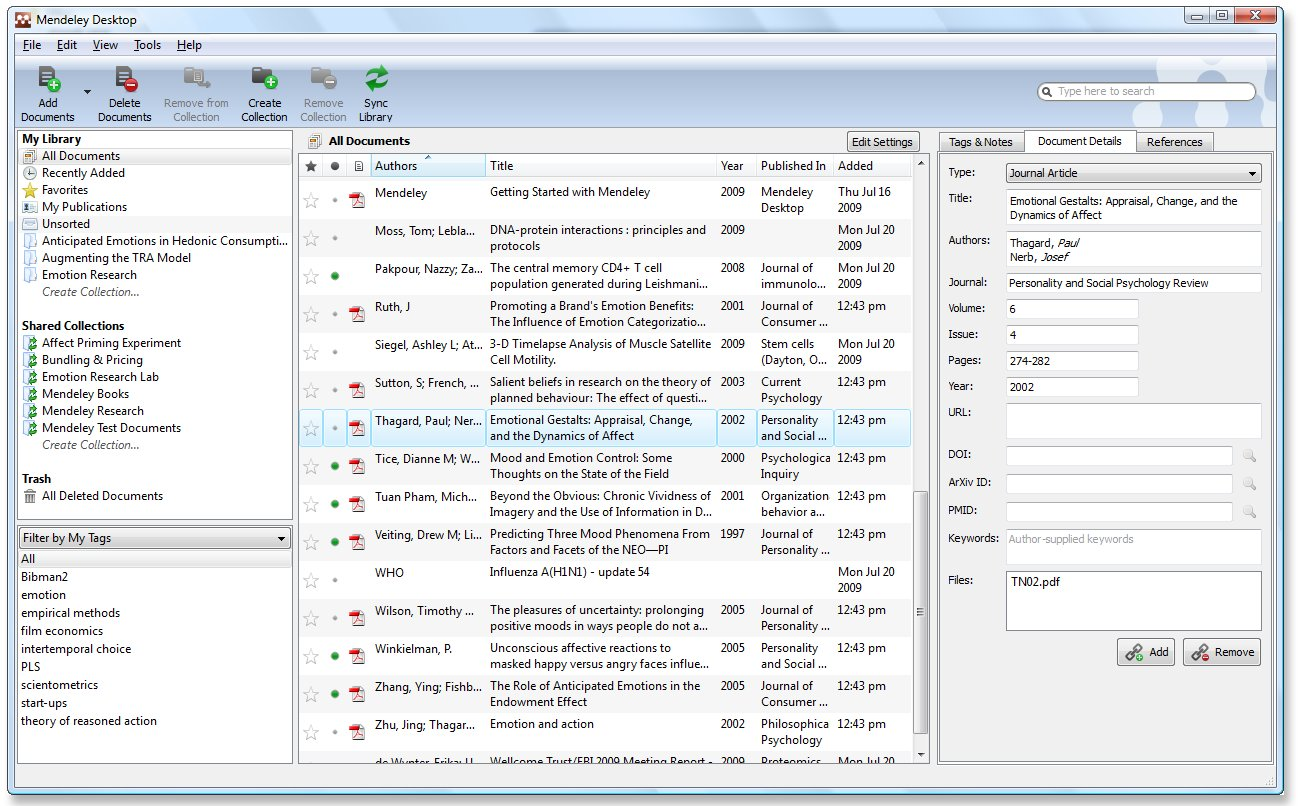
\includegraphics[width=1\textwidth]{img/Mendeley-destop-screenshot}\\ % Pfad
\source{\url{http://dominique-fleury.com/?p=302}} % Quelle
\end{minipage}
\end{figure}

\subsection{Texteditor}

Als Texteditor für \LaTeX wird Sublime Text (\url{http://www.sublimetext.com}) empfohlen. Zur Arbeit mit Latex ist das Plugin \emph{LaTeXTools} erforderlich (\url{https://github.com/SublimeText/LaTeXTools}).

\begin{figure}[hbt]
\centering
\begin{minipage}[t]{1\textwidth} % Breite, z.B. 1\textwidth		
\caption{Sublime Texteditor} % Überschrift
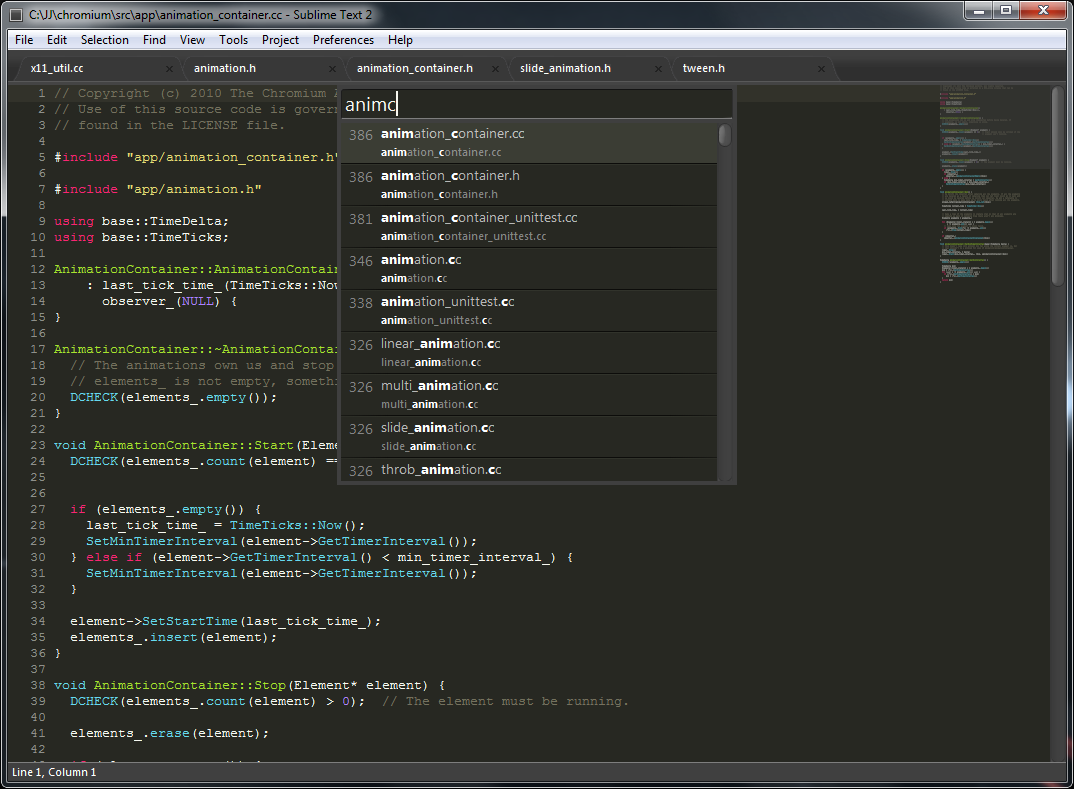
\includegraphics[width=1\textwidth]{img/sublime.png}\\ % Pfad
\source{\url{http://www.sublimetext.com/screenshots/alpha_goto_anything2_large.png}} % Quelle
\end{minipage}
\end{figure}

\subsection{PDF-Erzeugung}

Für die Erzeugung des PDF-Dokuments inklusive Referenzen, Quellenverzeichnis und Glossar sind mehrere Programmaufrufe und -durchläufe erforderlich. Der vollständige Aufruf zur PDF-Erzeugung lautet: 

\texttt{pdflatex Thesis}\\
\texttt{biber Thesis}\\
\texttt{makeindex -s Thesis.ist -t Thesis.alg -o Thesis.acr Thesis.acn}\\
\texttt{makeglossaries Thesis}\\
\texttt{pdflatex Thesis}\\
\texttt{pdflatex Thesis}\\

%!TEX root = ../Thesis.tex
\section{Grundlagen}

\subsection{Schrift}
\label{sec:schrift}

\subsubsection{Schriftgrößen}
\label{sec:schriftgroessen}
\tiny Das ist sehr kleine Schrift\\
\small Das ist kleine Schrift\\
\normalsize Das ist normale Schrift\\
\large Das ist große Schrift\\
\Large Das ist größere Schrift\\
\LARGE Das ist noch größere Schrift\\
\huge Das ist riesige Schrift\\
\Huge Das ist noch riesigere Schrift\\
\scriptsize Das ist Script Schrift\\
\footnotesize Das ist Fußnoten Schrift
\normalsize

\subsubsection{Schrift Typen}
\label{sec:Schrift Typen}
\textbf{Das ist ein fetter Text}\\
\textit{Das ist ein kursiver Text}\\
\underline{Das ist ein unterstrichener Text}\\
\textsc{Das ist ein kapitälchen Text}\\
\textsf{Das ist ein serifenloser Text}\\
\texttt{Das ist ein Schreibmaschinen Text}\\
\textnormal{Das ist ein normaler Text}

\subsubsection{Schrift Ausrichtung}
\label{sec:Schrift Ausrichtung}
\begin{quote}
Quote Text (Der gesamte Text innerhalb der Umgebung wird von beiden Seiten eingerückt)
\end{quote}
\begin{center}
Zentrierter Text (Der gesamte Text innerhalb der Umgebung wird zentriert)
\end{center}
\begin{flushleft}
Linksbündiger Text (Der gesamte Text innerhalb der Umgebung wird linksbündig)
\end{flushleft}
\begin{flushright}
Rechtsbündiger Text (Der gesamte Text innerhalb der Umgebung wird rechtsbündig)
\end{flushright}
In einer Fußnote\footnote{können zusätzliche Ergänzungen, Präzisierungen, Textverweise usw. eingeführt werden.}

\subsection{Abbildungen}

In \cref{fig:fhdw} sehen Sie das Logo der FHDW.

\begin{figure}[hbt]
\centering
\begin{minipage}[t]{.7\textwidth} % Breite, z.B. 1\textwidth		
\caption{Das Logo der FHDW} % Überschrift

\includegraphics[width=1\textwidth]{img/fhdw.pdf}\\ % Pfad
\source{Eigene Darstellung} % Quelle
\label{fig:fhdw}
\end{minipage}
\end{figure}

\subsection{Tabellen}

In \cref{tab:pin} auf Seite \pageref{tab:pin} sehen Sie die am häufigsten benutzten PINs.

\begin{table}[hbt]
\centering
\begin{minipage}[t]{.5\textwidth} % Breite, z.B. 1\textwidth		
\caption{Die am häufigsten verwendeten PINs} % Überschrift
\begin{tabularx}{\columnwidth}{rXrr}
\toprule
Rank & PIN & Percentage & Accumulated \\
\midrule
1 & 1234 & 4.34\% & 4.34\%\\
2 & 0000 & 2.57\% & 6.91\%\\
3 & 2580 & 2.32\% & 9.23\%\\
4 & 1111 & 1.60\% & 10.83\%\\
5 & 5555 & 0.87\% & 11.70\%\\
6 & 5683 & 0.70\% & 12.39\%\\
7 & 0852 & 0.60\% & 12.99\%\\
8 & 2222 & 0.56\% & 13.55\%\\
9 & 1212 & 0.49\% & 14.03\%\\
10 & 1998 & 0.43\% & 14.46\%\\
\bottomrule
\end{tabularx}
\source{Eigene Darstellung} % Quelle
\label{tab:pin}
\end{minipage}
\end{table}

\subsection{Zitate}

Ein Zitat im Fließtext ist zu sehen bei \citet{Fuller2011}.

Ein vergleichendes Zitat.\footnote{\cite[vgl.][5\psqq]{Maslennikov2011}}

Ein \enquote{wörtliches Zitat}\footnote{\cite[13\psq]{Meier2010}}

Zitat einer Quelle mit mehreren Autoren.\footnote{\cite[vgl.][32\psqq]{Hocking2011a}}


\subsection{Abkürzungen}
Bei der ersten Verwendung werden Abkürzungen ausgeschrieben: \gls{AES}.
Später wird dann automatisch nur noch die Kurzform benutzt: \gls{AES}


\subsection{Listen}
\label{sec:Listen}
Eine einfache List mit Punkten:

\begin{compactitem}
	\item Punkt 1
	\item Punkt 2
	\item Punkt 3
\end{compactitem}

Eine einfache Liste mit Nummern:
\begin{compactenum}
	\item Punkt 1
	\item Punkt 2 
	\item Punkt 3
\end{compactenum}

Eine einfache Liste mit römischen Nummern:
\begin{compactenum}[I.]
	\item Punkt 1
	\item Punkt 2
	\item Punkt 3
\end{compactenum}

Eine einfache Liste mit Buchstaben:
\begin{compactenum}[(a)]
	\item Punkt 1
	\item Punkt 2 
	\item Punkt 3
\end{compactenum}

\subsection{Quelltext}

Listing~\ref{list:android} auf Seite~\pageref{list:android} zeigt einigen Quelltext.

\begin{figure}[bht]
\begin{lstlisting}[caption=Scanning for Wi-Fi Access Points on Android, label=list:android]
registerReceiver(new RSSIBroadcastReceiver(), 
    new IntentFilter(WifiManager.SCAN_RESULTS_AVAILABLE_ACTION));

WifiManager wifi = getSystemService(Context.WIFI_SERVICE);
wifi.startScan();

/* not thread safe */
public class RSSIBroadcastReceiver extends BroadcastReceiver {

    public void onReceive(Context context, Intent intent) {
        WifiManager wifi = getSystemService(Context.WIFI_SERVICE);
        List<ScanResult> scanResults = wifiManager.getScanResults();

        for (ScanResult scanResult : results) {
            RSSI rssi = new RSSI();
            rssi.bssi = scanResult.BSSID;
            rssi.signalLevel = scanResult.level;
        }
    }
}
\end{lstlisting}
%\footnoterule{}
%\footnotesize{Casts have been omitted for the sake of readability}
\end{figure}

%!TEX root = ../Thesis.tex
\section{Zusammenfassung}

Dieses Dokument ist eine Hilfe, um die Formalien für eine Bachelor-Thesis an der
FHDW bei der Verwendung von {\LaTeX} zu erfüllen und dabei möglichst viele Automatismen von {\LaTeX} zu nutzen. Eine Absprache mit dem betreuenden Professor ist dennoch ratsam.

	
%%%%%%%%%%%%%%%%%%%%%%%%%%%%%%%%%%%%%%%%%%%%%%%%%%%%%%%%%%%%%%%%%%%%%%%

%!TEX root = ../Thesis.tex
\section*{Anhang}
\addcontentsline{toc}{section}{Anhang}
\fancyhead[R]{Anhang}

\anhangsverzeichnis

\anhang{Gesprächsnotizen}

\subanhang{Gespräch mit Werner Müller}

Gespräch mit Werner Müller am 01.01.2013 zum Thema XXX:
\begin{compactitem}
   \item Über das gute Wetter gesprochen
   \item Die Regenwahrscheinlichkeit liegt immer bei ca. 3\%
   \item Das Unternehmen ist total super
   \item Hier könnte eine wichtige Gesprächsnotiz stehen
\end{compactitem}


%!TEX root = ../Thesis.tex
\section*{Quellenverzeichnis}
\addcontentsline{toc}{section}{Quellenverzeichnis}
\fancyhead[R]{Quellenverzeichnis}

\defbibheading{mono}{\subsection*{Monographien}}
\defbibheading{mag}{\subsection*{Aufsätze in Sammelbänden und Zeitschriften}}
\defbibheading{art}{\subsection*{Zeitungsartikel}}
\defbibheading{web}{\subsection*{Internetquellen}}
\defbibheading{leg}{\subsection*{Rechtsprechung}}
\defbibheading{comp}{\subsection*{Unternehmensunterlagen/Gesprächsnotizen}}

\setlength\bibitemsep{1.5\itemsep}
\setlength{\bibhang}{2em}

\renewcommand{\baselinestretch}{1.50}\normalsize

\begingroup
\sloppy

\printbibliography[heading=mono,keyword=mono]
\printbibliography[heading=mag,keyword=mag]
\printbibliography[heading=web,keyword=web]

% Bei Bedarf einkommentieren: (erzeugt sonst Warnungen)
% \printbibliography[heading=art,keyword=art]
% \printbibliography[heading=leg,keyword=leg]
% \printbibliography[heading=comp,keyword=comp]

\endgroup


%%%%%%%%%%%%%%%%%%%%%%%%%%%%%%%%%%%%%%%%%%%%%%%%%%%%%%%%%%%%%%%%%%%%%%%

%!TEX root = ../Thesis.tex

\section*{Ehrenwörtliche Erklärung}
\addcontentsline{toc}{section}{Ehrenwörtliche Erklärung}
\fancyhead[R]{Ehrenwörtliche Erklärung}

Hiermit erkläre ich, dass ich die vorliegende \dokumententyp{} selbständig angefertigt habe. Es wurden nur die in der Arbeit ausdrücklich benannten Quellen und Hilfsmittel benutzt. Wörtlich oder sinngemäß übernommenes Gedankengut habe ich als solches kenntlich gemacht. Diese Arbeit hat in gleicher oder ähnlicher Form noch keiner Prüfungsbehörde vorgelegen.
\vspace{20mm}

\ort, \abgabedatum
\vspace{10mm}

\underline{\hspace{8cm}}\\\dokumentenautor
 
%%%%%%%%%%%%%%%%%%%%%%%%%%%%%%%%%%%%%%%%%%%%%%%%%%%%%%%%%%%%%%%%%%%%%%%

\end{document}